\documentclass[a4paper, 20pt,reqno]{article}
\usepackage[left=2cm,right=2cm,top=2cm,bottom=2cm]{geometry}
\usepackage[T2A]{fontenc}
% \DeclareMathSizes{10}{10}{10}{10}

\usepackage[russian]{babel}
\usepackage{soul}
\usepackage{gensymb}
\usepackage{amsfonts,amsmath,amssymb}
\usepackage{mathrsfs}
\usepackage{graphicx}
\usepackage[normalem]{ulem}
\usepackage[document]{ragged2e}
\usepackage{stmaryrd}
\usepackage{wrapfig}
\usepackage{fancyhdr}
\usepackage{floatflt}
\usepackage{python}
\usepackage{float}
\usepackage{amssymb}
\usepackage[most]{tcolorbox}
\usepackage{indentfirst}
\usepackage{setspace}
\usepackage{scrextend}
\usepackage{listings}
\usepackage{makecell,tabularx}
\usepackage{hyperref}
\usepackage{xcolor}

\newcommand{\mycopyright}{pluttan}
\newcommand{\docopyright}{$\mathfrak{Copyright}\ \mathfrak{\mycopyright} \logo$}
\newcommand{\rub}{{\rm{Р}\kern-.635em\rule[.5ex]{.52em}{.04em}\kern.11em}}

\definecolor{linkcolor}{HTML}{000000} 
\definecolor{urlcolor}{HTML}{0000FF} 

\hypersetup{pdfstartview=FitH,  linkcolor=linkcolor,urlcolor=urlcolor, colorlinks=true}

\definecolor{grey}{RGB}{40, 40, 40}

\renewcommand{\href}[1]{\url{#1}}

\definecolor{codegreen}{rgb}{0,0.6,0}
\definecolor{codegray}{rgb}{0.5,0.5,0.5}
\definecolor{codepurple}{rgb}{0.7,0,0.82}
\definecolor{mermaid}{rgb}{0.5,0.3,1}
\definecolor{backcolour}{rgb}{0.95,0.95,0.92}

\lstdefinestyle{mystyle}{
    backgroundcolor=\color{backcolour},   
    commentstyle=\color{codegreen},
    keywordstyle=\color{mermaid},
    numberstyle=\tiny\color{codegray},
    stringstyle=\color{codepurple},
    basicstyle=\ttfamily\footnotesize,
    breakatwhitespace=false,         
    breaklines=true,                 
    captionpos=b,                    
    keepspaces=true,                 
    numbers=left,                    
    numbersep=5pt,                  
    showspaces=false,                
    showstringspaces=false,
    showtabs=false,                  
    tabsize=2,
  extendedchars=true , % включаем не латиницу 
  escapechar=|, % |«выпадаем» в LATEX|
  frame=tb , % рамка сверху и снизу 
  commentstyle=\itshape , % шрифт для комментариев 
  stringstyle=\bfseries
}

\lstset{style=mystyle}

\lstdefinestyle{CommentStyle}{
    language=XML,
    %numbers=left, numberstyle=\tiny, stepnumber=1, numbersep=5pt,
    commentstyle=\color{red},
	basicstyle=\footnotesize\ttfamily,
	language={[ANSI]C++},
	keywordstyle=\bfseries,
	showstringspaces=false,
	morekeywords={include, printf},
	commentstyle={},
	escapeinside=§§,
	escapebegin=\begin{russian}\commentfont,
	escapeend=\end{russian},
    keywordstyle=\color{blue}\bfseries,
    morekeywords={align,begin},
    extendedchars=\true,
    tabsize=2
}
\lstdefinestyle{myLatexStyle}{
    language=c++,
    %backgroundcolor=\color{grey},
    numbers=left, numberstyle=\tiny, stepnumber=1, numbersep=5pt,
    commentstyle=\color{red},
    keywordstyle=\color{blue}\bfseries,
    morekeywords={align,begin},
    extendedchars=\true,
    tabsize=2
}

\lstdefinestyle{pmyLatexStyle}{
    language=java,
    %backgroundcolor=\color{grey},
    numbers=left, numberstyle=\tiny, stepnumber=1, numbersep=5pt,
    commentstyle=\color{red},
    keywordstyle=\color{blue}\bfseries,
    morekeywords={align,begin},
    extendedchars=\true,
    tabsize=2
}

\definecolor{block-gray}{gray}{0.90} % уровень прозрачности (1 - максимум)
\definecolor{yellow}{HTML}{F0FFFF}
\newtcolorbox{myquote}{colback=block-gray,grow to right by=-10mm,grow to left by=-10mm,boxrule=0pt,boxsep=0pt,breakable} % настройки области с изменённым фоном
\newtcolorbox{myquote2}{colback=yellow,grow to right by=-10mm,grow to left by=-10mm,boxrule=0pt,boxsep=0pt,breakable} % настройки области с изменённым фоном

\setlength{\parindent}{12,5mm}

\newcommand{\logo}{\vcenter{\hbox{
\includegraphics[width=.8em]{/Users/pluttan/Documents/bw2.png}}}}
\onehalfspacing

\pagestyle{fancy}
\renewcommand{\sectionmark}[1]{\markright{#1}}
\fancyhf{} 
\fancyhead[R]{\bfseries\thepage}
\fancyhead[LO]{\docopyright}

\newcommand{\image}[2]{
	\begin{figure}[H]
		\center{\includegraphics[height=#2pt]{../img/#1} }
    \end{figure}
}

\newcommand{\dotitle}[2]{

\thispagestyle{empty}
\sloppy{
  \scriptsize{
    \line(6,0){0}

    \centering \docopyright

    \centering Привет! Меня зовут Андрей, я создаю свою ботву, этот файл малая ее часть. 
    
    \centering Пользоваться и распространять файлы конечно же можно. Если вы нашли ошибку в файле, можете 
    
    \centering исправить ее в исходном коде и подать на слияние или просто написать в issue. 

    \centering {\bf{Так же вы можете купить распечатанную версию данного файла в виде книжки.}
    
    \centering По всем вопросам писать в ВК.}
    
    \centering Приятного бота)

    \line(6,0){300}

    \centering GitHub: \href{https://github.com/pluttan}

    \centering VK: \href{https://vk.com/pluttan}

    \line(6,0){0}
  }}

\begin{figure}[H]
		\center{\includegraphics[height=100pt]{/Users/pluttan/Documents/forMyDocs/qr2.png} }
\end{figure}

\topskip=-200pt
\vspace*{130pt}
\begin{Huge}
  \textbf{
    \begin{center}
        #1
    \end{center}
  }
  {\begin{center} 
        #2
    \end{center}}
\end{Huge}
\vspace*{300pt}
  \begin{flushright}
    Над файлом работали: \\
    \mycopyright
  \end{flushright}
\newpage
\pagestyle{fancy}
\renewcommand{\sectionmark}[1]{\markright{#1}}
\fancyhf{} 
\fancyhead[R]{\bfseries\thepage}
\fancyhead[LO]{\docopyright}
}
\renewcommand{\sectionmark}[1]{\markright{#1}}
\renewcommand{\sectionmark}[1]{\markright{#1}}
% \makeatletter
%      \renewcommand*\l@section{\@dottedtocline{1}{0em}{1.8em}}
%      \renewcommand*\l@subsection{\@dottedtocline{2}{1.5em}{2.0em}}
%      \renewcommand*\l@subsubsection{\@dottedtocline{3}{4.3em}{3.0em}}
% \makeatother
\newcommand{\toc}{
\newpage
\renewcommand{\contentsname}{Оглавление}
\large{\tableofcontents}
\newpage
\large
}


% It's XeLaTeX, if you can't compile comment this line 
\usepackage{fontspec}\setmainfont{Times New Roman} 

\renewcommand{\dotitle}[2]{

\thispagestyle{empty}
\begin{minipage}[l]{300pt}
  \vspace*{25pt}
  \sloppy{
  \scriptsize{
    \line(6,0){0}

    \centering \docopyright

    \centering Привет! Это Трубусы и Уточки, мы создаем свою ботву, этот файл малая ее часть. 
    
    \centering Пользоваться и распространять файлы конечно же можно. Если вы нашли ошибку в файле, можете 
    
    \centering исправить ее в исходном коде и подать на слияние или просто написать в issue. 

    \centering \textbf{Так же вы можете купить распечатанную версию данного файла в виде книжки.}
    
    \centering \textbf{По всем вопросам писать в ВК.}
    
    \centering Приятного бота)

    \line(6,0){300}

    \centering GitHub: \href{https://github.com/pluttan}

    \centering VK: \href{https://vk.com/pluttan}

    \centering VK: \href{https://vk.com/f_i_i_x_i_i}

    \line(6,0){0}}
}
\end{minipage}
\begin{minipage}[r]{150pt}
  \raggedright
\includegraphics[height=150pt]{/Users/pluttan/Documents/forMyDocs/qr1.png}
\end{minipage}


\topskip=-250pt
\vspace*{170pt}
\begin{Huge}
  \textbf{
    \begin{center}
        #1
    \end{center}
  }
  {\begin{center} 
        #2
    \end{center}}
\end{Huge}
\vspace*{250pt}
  \begin{flushright}
    Над файлом работали: \\
    \mycopyright
  \end{flushright}
% \newpage
\pagestyle{fancy}
\renewcommand{\sectionmark}[1]{\markright{#1}}
\fancyhf{} 
\fancyhead[R]{\bfseries\thepage}
\fancyhead[LO]{\docopyright}
}
\renewcommand{\mycopyright}{pluttan \& fiixii}

\usepackage{titlesec}
\titleformat{\section}
  {\fontsize{18}{15}\bfseries}{\thesection}{1em}{}
\titleformat{\subsection}
  {\tt\fontsize{16}{15}\bfseries}{\thesubsection}{1em}{}

\newcommand{\hlek}[1]{{\normalsize\begin{center}\textit{Л.С. Сеченкова, Н.В. Палий Начертательная геометрия Лекционная тетрадь стр. #1}\end{center}}}
\newcommand{\hbook}[1]{{\normalsize\begin{center}\textit{Б.Г. Жирных, В.И. Серегин, Ю.Э. Шарикян Начертательная геометрия стр. #1}\end{center}}}


% It's XeLaTeX, if you can't compile:
% 1. download & install this https://isopromat.ru/wp-content/uploads/fonts-GOST.zip
% 2. try to use XeLaTeX 
% OR comment this line 

%%%%%%%%%%%%%%%%%%%%%%%%%%%%%%%%%%%%%%%%%%%%%%%%%%%%%%%%%%%%%%%%
%значения комментариев
%! Forced transition - вынужденный переход на новую страницу
%%%%%%%%%%%%%%%%%%%%%%%%%%%%%%%%%%%%%%%%%%%%%%%%%%%%%%%%%%%%%%%%
\begin{document}
\setmonofont{GOST Type BU}
\tikz[remember picture,overlay] \node[opacity=0.1,inner sep=0pt] at (current page.center){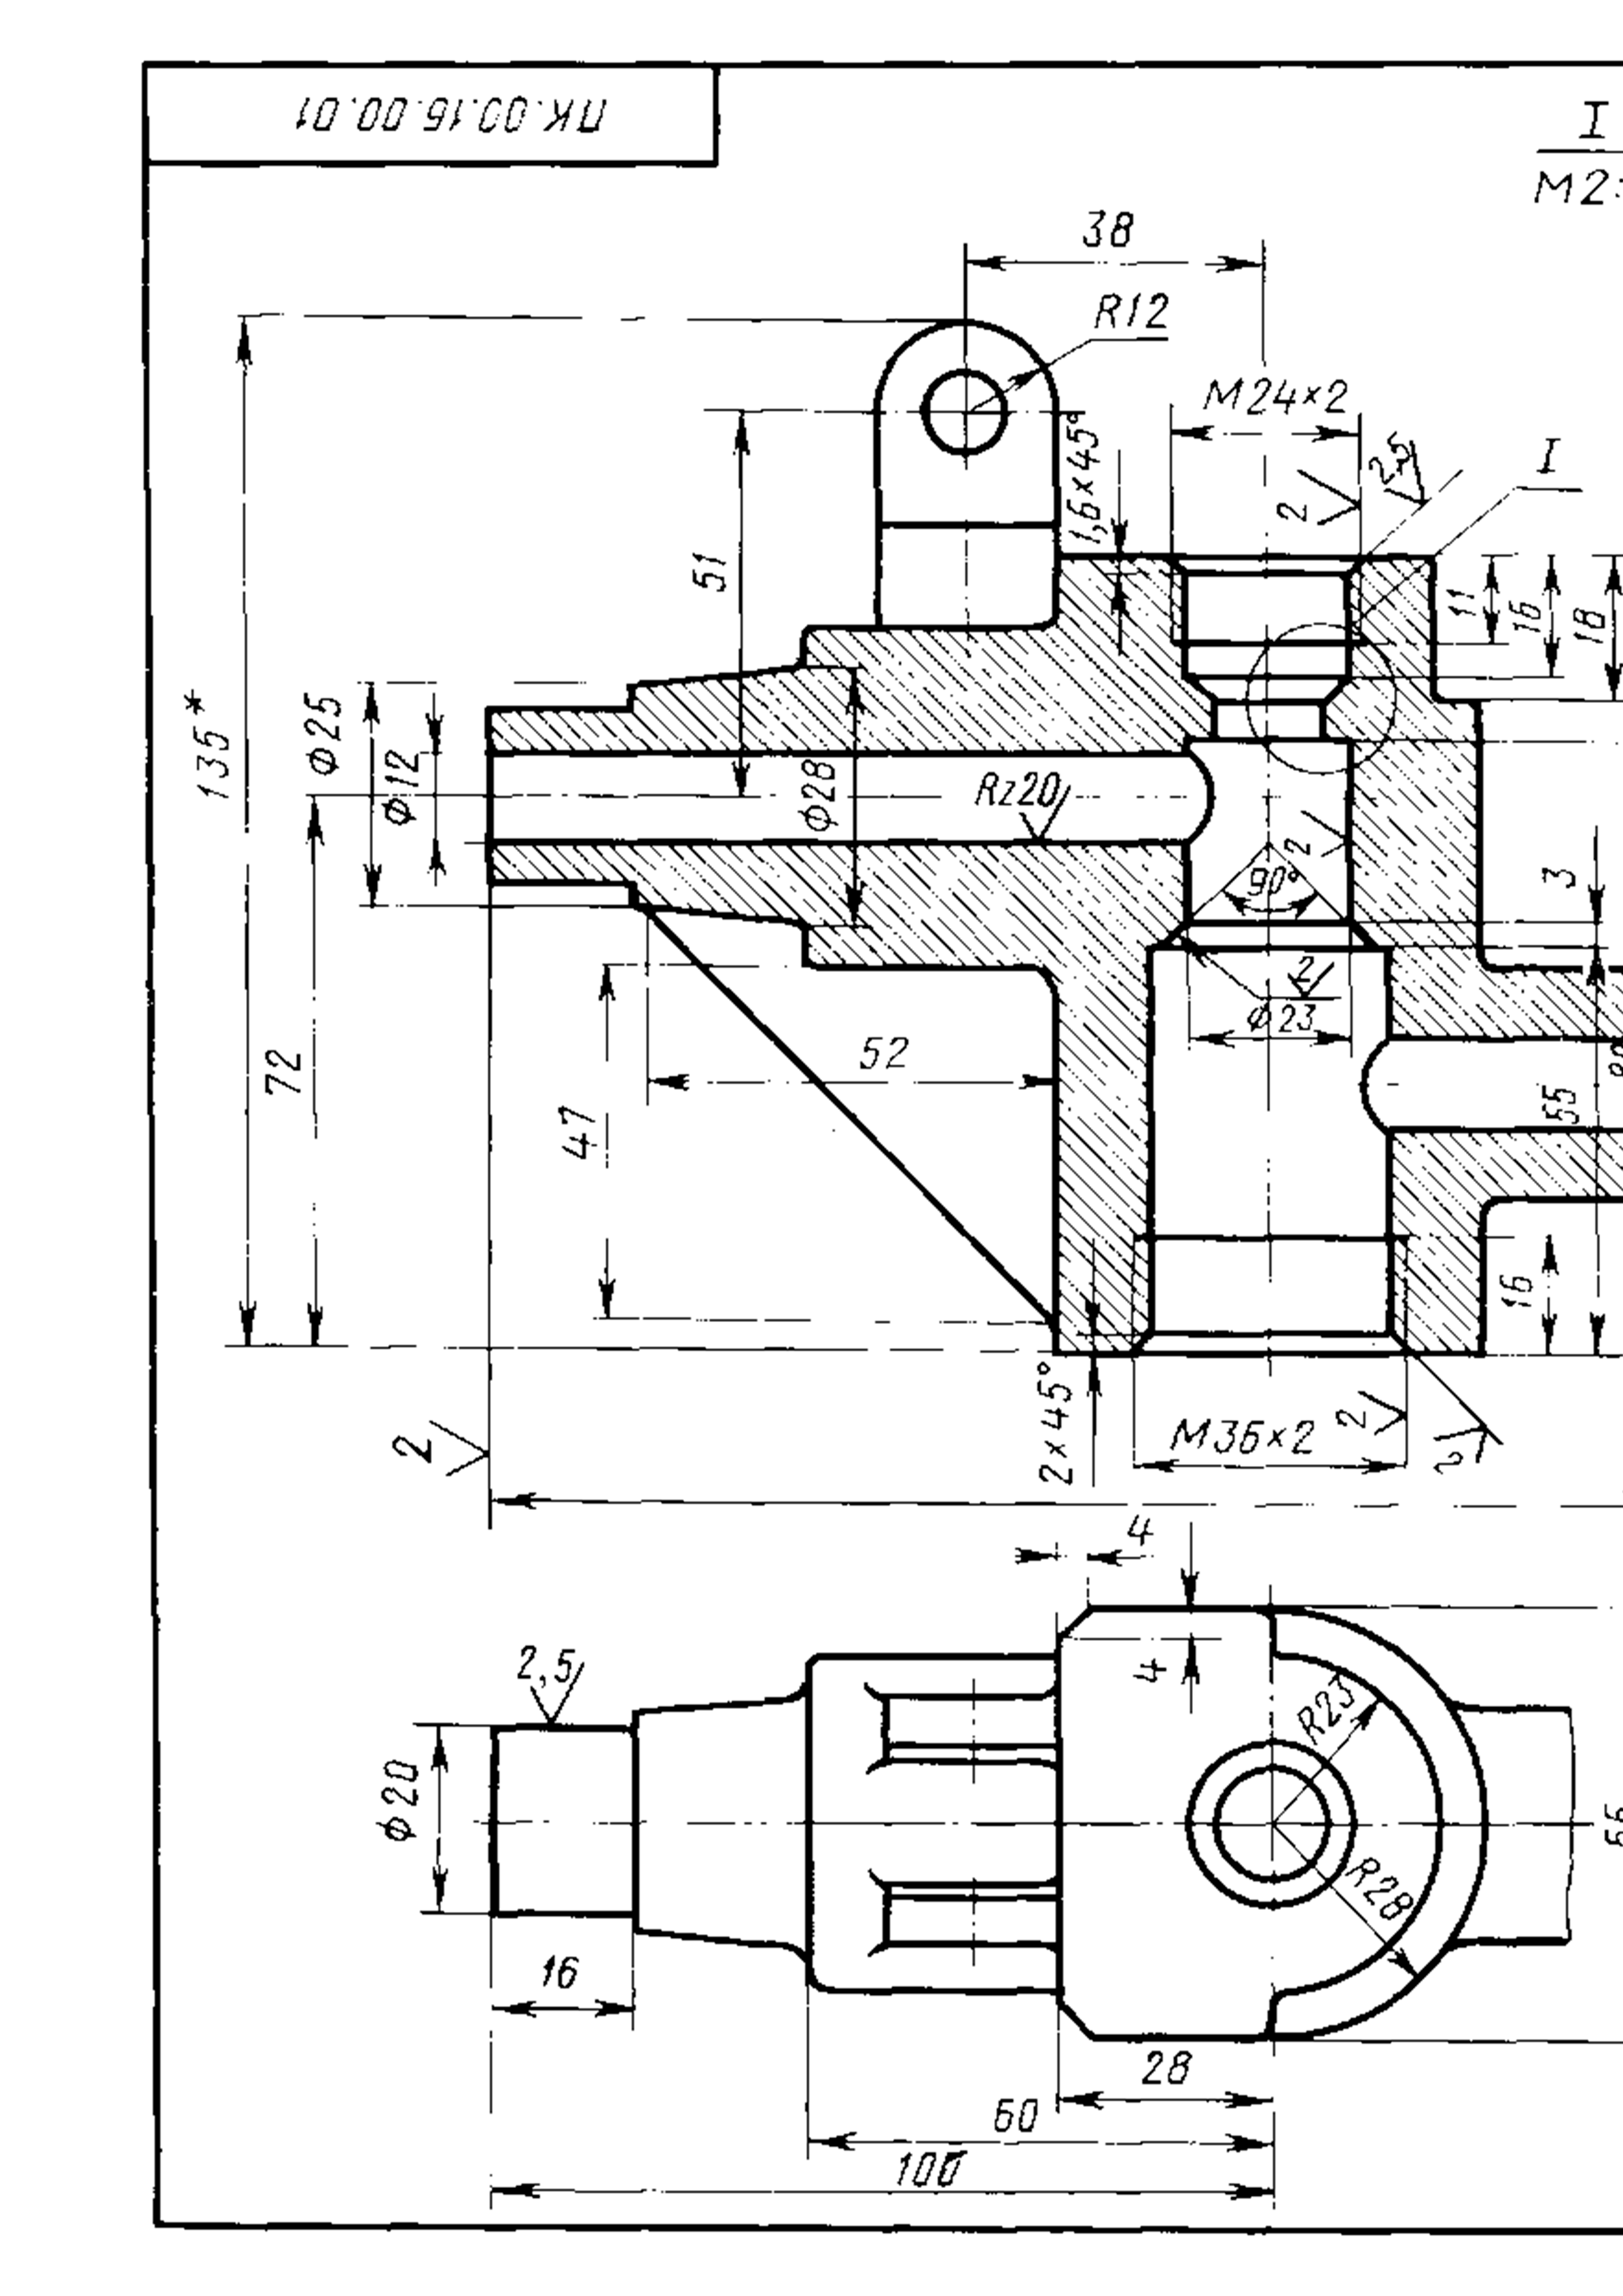
\includegraphics[width=\paperwidth,height=\paperheight]{../img/bg2.png}};
\dotitle{\texttt{Подготовка к экзамену}}{\texttt{Начертательная геометрия}}{}
\toc
\large
\section{Теория}

%-------------------------
%       Вопрос 1
%-------------------------

\subsection{\texttt{Свойства прямоугольного проецирования}}

\begin{myquote}
    \hlek{6}
    
    \hbook{16 - 20}
\end{myquote}

\begin{enumerate}
    \item Проекция точки есть точка.% ебнешься, да?)

    \image{1Point.jpg} {150}

    \item В общем случае проекция прямой есть прямая линия, проекция кривой линии есть кривая.

    \item Свойство принадлежности: при проецировании сохраняется принадлежность точки $A$ линии $l$: если $A \in l$, то $A' \in l'$.

    \image{1Property2.jpg} {150}

    \item Параллельные прямые проецируются в парралельные прямые.

    \image{1Property3.jpg} {150}
    \item Сохраняется простое отношение трех точек, т.е. {\Large $\frac{AB}{BC} = \frac{A'B'}{B'C'}$}.

    \image{1property5.jpg} {150}

\end{enumerate}


Для выполнения чертежей важно отметить следующие свойства:

\begin{enumerate}
    \item Если плоская фигура параллельна плоскоскости проекций, то она проецируется на эту плоскость без искажений.
    
    \image{1property2_2.jpg}{150}
    
    \item При параллельном переносе плоскости проекций в направлении проецирования проекции фигуры остаются неизменными.
    
\end{enumerate}

%-------------------------
%       Вопрос 2
%-------------------------

\newpage
\subsection{\texttt{Какие линии называются проецирующими линиями, линиями уровня?}}

\begin{myquote}
    \hlek{8 - 9}
    
    \hbook{28 - 30}
\end{myquote}

Прямые, перпендикулярные плоскостям проекций, называются {\bf проецирующими
линиями}. Такие прямые проецируются в точку на ту плоскость проекций, которой эта
прямая перпендикулярна.

Выделяют следующие виды проецирующих прямых:
\begin{enumerate}
    \item \textit {Горизонтально-проецирующая прямая} (прямая перпендикулярна горизонтальной плоскости проекций).
    
    \image{2Horisontal.jpg}{150}

    \item \textit{Фронтально-проецирующая прямая} (прямая перпендикулярна фронтальной плоскости проекций).

    \image{2Frontal.jpg}{150}

    \item \textit {Профильно-проецирующая прямая} (прямая перпендикулярна профильной плоскости проекций).

    \image{2Profile.jpg}{150}

\end{enumerate}


Прямые, параллельные плоскостям проекций, называются {\bf прямыми
уровня}.

Выделяют следующие виды прямых уровня:
\begin{enumerate}
    \item \textit {Горизонтальная прямая} (прямая параллельна горизонтальной плоскости проекций).
    
    \image{2HorisontalPar.jpg}{150}

    \item \textit {Фронтальная прямая} (прямая параллельна фронтальной плоскости проекций).

    \image{2FrontalPar.jpg}{150}

    \item \textit {Профильная прямая} (прямая параллельна профильной плоскости проекций).

    \image{2ProfilePar.jpg}{150}

\end{enumerate}

%-------------------------
%       Вопрос 3
%-------------------------

\newpage
\subsection{\texttt{Какие линии, принадлежащие плоскости, называются горизонталью, фронталью?}}

\begin{myquote}
    \hlek{12 - 13}
    
    \hbook{46 - 48}
\end{myquote}

{\bf Горизонталью плоскости} называется прямая, принадлежащая данной плоскости и параллельная горизонтальной плоскости проекций.

\image{horisontal.png}{170}

{\bf Фронталью плоскости} называется прямая, принадлежащая данной плоскости и параллельная фронтальной плоскости проекций.

\image{frontal.png}{170}

%-------------------------
%       Вопрос 4
%-------------------------

\newpage
\subsection{\texttt{Теорема о проецировании прямого угла}}

\begin{myquote}
    \hlek{10}
\end{myquote}

Если одна сторона прямого угла параллельна плоскости проекций, а вторая сторона не перпендикулярна к ней, то прямой угол проецируется без искажения на данную плоскость проекций.

\image{4Teor.jpg}{250}

%-------------------------
%       Вопрос 5
%-------------------------

\newpage
\subsection{\texttt{На основании каких положений строят перпендикулярные: прямую и плоскость?}}

\begin{myquote}
    \hlek{14}
    
    \hbook{50}
\end{myquote}

Построение на чертеже {\bf перпендикулярных} прямой и плоскости основано на использовании:

\begin{enumerate}
    \item \textit {признака перпендикулярности прямой и плоскости}: прямая перпендикулярна плоскости, если она перпендикулярна двум пересекающимся прямым, принадлежащим этой плоскости;
    \item \textit {теоремы о проекциях прямого угла}.
\end{enumerate}


%-------------------------
%       Вопрос 6
%-------------------------

\newpage
\subsection{\texttt{На основании каких положений строят параллельные: прямую и плоскость?}}

\begin{myquote}
    \hlek{13}
    
    \hbook{49}
\end{myquote}

Построение на чертеже {\bf параллельных} прямой и плоскости основано на:

\begin{enumerate}
    \item Использовании \textit {признака параллельности прямой и плоскости}: прямая параллельна плоскости, если она параллельна прямой, принадлежащей этой плоскости;
    \item Использовании \textit {свойства проецирования параллельных прямых}: если прямые параллельны, то и проекции этих прямых параллельны.
\end{enumerate}



%-------------------------
%       Вопрос 7
%-------------------------

\newpage
\subsection{\texttt{На основании каких положений строят на чертеже две параллельные плоскости?}}

\begin{myquote}
    \hlek{14}
    
    \hbook{49}
\end{myquote}

Построение на чертеже {\bf параллельных} плоскостей основано на:

\begin{enumerate}
    \item Использовании \textit {признака параллельности двух плоскостей}: две плоскости параллельны, если две пересекающиеся прямые одной плоскости параллельны двум пересекающимся прямым другой плоскости;
    \item Использовании \textit {свойства проецирования параллельных прямых}: если прямые параллельны, то и проекции этих прямых параллельны.
\end{enumerate}

%-------------------------
%       Вопрос 8
%-------------------------

\newpage
\subsection{\texttt{На основании каких положений строят на чертеже две перпендикулярные плоскости?}}

\begin{myquote}
    \hlek{15}
    
    \hbook{50 - 51}
\end{myquote}

Построение на чертеже {\bf перпендикулярных} плоскостей основано на:
\begin{enumerate}
    \item использовании \textit {признака перпендикулярности двух плоскостей}: две плоскости взаимно перпендикулярны, если одна из этих плоскостей содержит прямую, перпендикулярную к другой плоскости;
    \item использовании \textit {теоремы о проекциях прямого угла}.
\end{enumerate}



%-------------------------
%       Вопрос 9 
%-------------------------

\newpage
\subsection{\texttt{Правило построения проекции точки, принадлежащей поверхности}}

\begin{myquote}
    \hlek{19}
\end{myquote}

Общее правило построения проекций точки, принадлежащей поверхности:

Для построения проекции точки, принадлежащей поверхности, надо воспользоваться проекциями линии, {\bf принадлежащей поверхности} и {\bf проходящей через заданную точку}. 

%-------------------------
%       Вопрос 10
%-------------------------

\newpage
\subsection{\texttt{Правило построения проекции точки, принадлежащей плоскости}}

\begin{myquote}
    \hlek{12}
    
    \hbook{45}
\end{myquote}

Общее правило построения проекции точки, принадлежащей плоскости:

Для построения проекции точки, принадлежащей плоскости общего положения, надо воспользоваться проекциями прямой, {\bf принадлежащей заданной плоскости} и {\bf проходящей через точку} (используем свойство принадлежности).


%-------------------------
%       Вопрос 11 %?check
%-------------------------

\newpage
\subsection{\texttt{Правило построения проекций точки, принадлежащей поверхности вращения}}

\begin{myquote}
    \centering Сформулировал F\_i\_i\_X\_i\_i
\end{myquote}

Общее правило построения проекций точки, принадлежащей поверхности вращения:

Для построения проекции точки, принадлежащей поверхности вращения, надо воспользоваться проекциями прямой, {\bf являющейся образующей поверхности} и {\bf проходящей через заданную точку}. 

%-------------------------
%       Вопрос 12
%-------------------------

\newpage
\subsection{\texttt{Способы преобразования}}

\begin{myquote}
    \hlek{24 - 32}
    
    \hbook{52 - 66}
\end{myquote}

Различают три способа преобразования:
\begin {enumerate}

\item {\bf Cпособ замены плоскостей проекций} - суть этого способа заключается в том, что в системе двух плоскостей проекций заменяют одну из плоскостей проекций на новую плоскость, перпендикулярную
неизменяемой плоскости проекций. На эту плоскость проецируют заданные
геометрические фигуры, которые в пространстве неподвижны.

\image{12ReplacePlanes.jpg}{150}

\item {\bf Cпособ плоскопараллельного перемещения} - суть этого способа заключается в том, что все точки геометрической фигуры перемещаются в
параллельных плоскостях.

\image{12ReplacePlanes2.jpg}{150}

\item {\bf Cпособ вращения (вокруг проецирующей прямой)} - суть этого способа заключается в том, что все точки фигуры движутся по окружностям в плоскостях, перпендикулярных к оси вращения (т.е. параллельно плоскости проекций, которой перпендикулярна ось вращения).

\image{12Rotation.jpg}{150}

\end {enumerate}



%-------------------------
%       Вопрос 13
%-------------------------

\newpage
\subsection{\texttt{Условия преобразования способом замены плоскостей проекций}}

\begin{myquote}
    \hlek{24 - 27}
    
    \hbook{52 - 58}
\end{myquote}

Условия преобразования:
\begin{enumerate}
    \item Положение фигуры неизменно;
    \item Изменяется положение одной из двух плоскостей проекций;
    \item Новую плоскость проекций располагают перпендикулярно оставшейся плоскости проекций;
    \item Положение новой плоскости проекций может быть задано или выбрано.
\end{enumerate}

%-------------------------
%       Вопрос 14
%-------------------------

\newpage
\subsection{\texttt{Условия преобразования способом вращения вокруг проецирующей прямой}}

\begin{myquote}
    \hlek{29 - 32}
    
    \hbook{63 - 66}
\end{myquote}

Условия преобразования:
\begin{enumerate}
    \item Ось вращения i неподвижна и перпендикулярна плоскости проекций;
    \item Все точки фигуры перемещаются по окружностям, плоскости которых перпендикулярны оси i;
    \item Точки, лежащие на оси i, неподвижны.
\end{enumerate}

%-------------------------
%       Вопрос 15 
%-------------------------

\newpage
\subsection{\texttt{Какая линия поверхности вращения называется меридианом, параллелью?}}

\begin{myquote}
    \hlek{20}
\end{myquote}
{\bf Меридиан} - это линия пересечения поверхности вращения с плоскостью, проходящей через ось вращения (такая плоскость называется \textit {меридиональной}).

{\bf Главным меридианом} называют меридиан, лежащий в плоскости уровня.

{\bf Параллель} - это окружность, описываемая точкой, лежащей на образующей, при ее вращении вокруг оси вращения. 
\begin{itemize}
    \item Центр параллели лежит на оси вращения; 
    \item Параллель лежит в плоскости, перпендикулярной оси вращения.
\end{itemize}

Наибольшая параллель называется {\bf экватором}, наименьшая - {\bf горлом}.

\image{15_1.jpg}{150}

%-------------------------
%       Вопрос 16 %?check
%-------------------------

\newpage
\subsection{\texttt{В какую линию может проецироваться окружность при разных ее положениях отностельно плоскостей проекций?}}

\begin{myquote}
    \hlek{17}
\end{myquote}
Окружность может проецироваться в:
\begin{itemize}
    \item {\bf окружность}, если плоскость проекции параллельна плоскости, в которой лежит окружность.
    \item {\bf прямую}, если плоскость проекции перпендикулярна плоскости, в которой лежит окружность.
    \item {\bf эллипс}, в остальных случаях.
\end{itemize}

\image{16_1.jpg}{150}

%-------------------------
%       Вопрос 17
%-------------------------

\newpage
\subsection{\texttt{Алгоритм построения точек пересечения линии с поверхностью}}
\begin{myquote}
    \hlek{39}
\end{myquote}
Алгоритм построения точек пересечения линии с поверхностью:
\begin{enumerate}
    \item заключить данную линию во вспомогательную поверхность $\gamma$;
    \item определить линию пересечения этой вспомогательной поверхности с заданной поверхностью;
    \item отметить точки, в которых пересекаются полученная линия с заданной.
\end{enumerate}

\image{17_1.jpg}{150}
%-------------------------
%       Вопрос 18 %?check
%-------------------------

\newpage
\subsection{\texttt{Последовательность построения точки пересечения прямой и плоскости}}
\begin{myquote}
    \hlek{40}
    \hbook{103}
\end{myquote}

Последовательность построения:
\begin{enumerate}
    \item заключаем данную прямую во вспомогательную проецирующую плоскость $\gamma$;
    \item строим проекции линии пересечения данной плоскости с плоскостью $\gamma$;
    \item строим проекции точки пересечения полученной линии с данной прямой.
Полученная в последнем пункте точка - и есть точка пересечения прямой и плоскости.
\end{enumerate}


%-------------------------
%       Вопрос 19
%-------------------------

%\newpage
%\subsection{\texttt{Последовательность построения точек пересечения прямой и %поверхности}}
\subsection{}


%-------------------------
%       Вопрос 20
%-------------------------

\newpage
\subsection{\texttt{Какие линии получаются в сечении цилиндрической поверхности плоскостью при разных положениях плоскости относительно оси цилиндрической поверхности?}}
\begin{myquote}
    \centering Сформулировал F\_i\_i\_X\_i\_i
\end{myquote}

\begin{enumerate}
    \item Секущая плоскость {\bf параллельна} оси цилинда:
    \begin{itemize}
        
        \item Расстояние от оси до секущей плоскости {\bf меньше} радиуса основания цилиндра: в сечении будет {\bf две образующие};
        \image{20_1_1.jpg}{250};

        \item Расстояние от оси до секущей плоскости {\bf равно} радиусу основания цилиндра: в сечении будет {\bf одна образующая}; 
        \image{20_1_2.jpg}{250};

        \item Расстояние от оси до секущей плоскости {\bf больше} радиуса основания цилиндра: секущая плоскость {\bf не пересекает} цилиндр;
        \image{20_1_1.jpg}{250};

    \end{itemize}
    \item Секущая плоскость пересекает ось цилиндра под углом $\alpha$ (0\textdegree < $\alpha$ <= 90\textdegree)
    \begin {itemize}

        \item Секущая плоскость {\bf параллельна} основаниям цилиндра: в сечении будет окружность;
        \image{20_2_1.jpg}{250};

        \item Секущая плоскость {\bf не пересекает ни одну окружность в основаниях цилиндра}: в сечении будет эллипс;
        \image{20_2_2.jpg}{250};

        \item Секущая плоскость {\bf пересекает одну или две окружности в основаниях цилиндра}: в сечении будет часть эллипса;
        \image{20_2_3.jpg}{250};

    \end{itemize}
    
\end{enumerate}
%-------------------------
%       Вопрос 21
%-------------------------

\newpage
\subsection{\texttt{Конические сечения. При каком положении плоскости относительно оси конической поверхности сечением является окружность, эллипс, прямые, парабола, гипербола?}}

\begin{myquote}
    \hlek{36}
\end{myquote}

\begin{enumerate}
    \item Секущая плоскость $\alpha$ {\bf не проходит через вершину конуса}:
    \begin{itemize}
        \item Секущая плоскость пересекает все образующие конуса и параллельна основанию: в сечении будет {\bf окружность};
        \image{21_1_1.jpg}{220}
        \item Секущая плоскость пересекает все образующие конуса и не параллельна основанию: в сечении будет {\bf эллипс};
        \image{21_1_2.jpg}{220}
        \item Секущая плоскость параллельна одной образующей конуса: в сечении будет {\bf парабола};
        \image{21_1_3.jpg}{220}
        \item Секущая плоскость параллельна двум образующим конуса: в сечении будет {\bf гипербола}.
        \image{21_1_4.jpg}{260}
    \end{itemize}
    \newpage %!Forced transition
    \item Секущая плоскость $\alpha$ {\bf проходит через вершину конуса}:
    \begin{itemize}
        \item Угол между секущей плоскостью и осью вращения {\bf меньше} чем угол между образующей и осью вращения: в сечении будет {\bf две образующие};
        \image{21_2_1.jpg}{250}
        \item Угол между секущей плоскостью и осью вращения {\bf равен} углу между образующей и осью вращения: в сечении будет {\bf одна образующая};
        \image{21_2_2.jpg}{250}
        \item Угол между секущей плоскостью и осью вращения {\bf больше} чем угол между образующей и осью вращения: в сечении {\bf будет точка};
        \image{21_2_3.jpg}{250}

    \end{itemize}
\end{enumerate}


%-------------------------
%       Вопрос 22
%-------------------------

\newpage
\subsection{\texttt{Последовательность построения линии пересечения двух поверхностей}}





%-------------------------
%       Вопрос 23
%-------------------------

\newpage
\subsection{\texttt{Теорема Монжа. Привести пример}}

\begin{myquote}
    \hlek{47}
    
    \hbook{127-128}
\end{myquote}

Если две поверхности второго порядка вписаны или описаны около третьей поверхности второго порядка, то они пересекаются по двум плоским кривым второго порядка. Плоские кривые проецируются в отрезки прямых линий на общую плоскость симметрии пересекающихся плоскостей. На чертеже эти отрезки прямых пересекаются в точке, которая является проекцией точек пересечения линий касания.

\image{23monz.jpg}{200}

%-------------------------
%       Вопрос 24
%-------------------------

\newpage
\subsection{\texttt{Какую плоскость называют касательной к поверхности в данной точке?}}

\begin{myquote}
    \hlek{48}
    
    \hbook{137-139}
\end{myquote}

Плоскость, образованная касательными прямыми к двум любым линиям поверхности, пересекающимися в заданной на поверхности точке, называется {\bf касательной к поверхности в данной точке}.

\image{24kas.jpg}{200}

%-------------------------
%       Вопрос 25
%-------------------------

\newpage
\subsection{\texttt{Что называется нормалью к поверхности в данной точке?}}

\begin{myquote}
    \hlek{48}
    
    \hbook{137-139}
\end{myquote}

{\bf Нормаль} $n$ поверхности в данной точке перпендикулярна к касательной плоскости в этой точке поверхности.

%для потомков ( Андрей старался :) )
%$\alpha$ - поверхность,
%$a \subset \alpha; b \subset \alpha; a \cub b \rightarrow A;$
%$t_1 \overline{\cup} a; t_2 \overline{\cup} a; t_1 \cap t_2 \rightarrow A; n \perp ( t_1 \cap t_2)$

\image{24kas.jpg}{200}

%-------------------------
%       Вопрос 26
%-------------------------

\newpage
\subsection{\texttt{Алгоритм решения задач на построение линии пересечения поверхностей, одна из которых занимает проецирующее положение}(Из другого файла)}

%-------------------------
%       Вопрос 27
%-------------------------

\newpage
\subsection{\texttt{Построение линии пересечения поверхностей с использованием вспомогательных плоскостей. Область применения способа}(Из другого файла)}


\end{document}